\section{数学部分的准备}

\subsection{傅里叶级数}

\begin{frame}
    \frametitle{傅里叶级数}
    在微积分3中,我们曾学过傅里叶级数。
    \begin{itemize}
        \item 傅里叶级数的实质,是将周期函数展开为正弦函数和余弦函数的叠加。
        \item 傅里叶级数中的系数,由周期函数的积分确定。
    \end{itemize}
\end{frame}

\begin{frame}
    \begin{theorem}[傅里叶级数]
        设$f(x)$是周期为$2L$的周期函数,即满足$f(x)=f(x+2L)$,且在$[-L,L]$上可积。

        若$f(x)$可以展开为以下形式的傅里叶级数
        \begin{equation}
            f(x)=a_0+\Sum[n=1][\infty]{a_n\cos\frac{n\pi}{L}x+b_n\sin\frac{n\pi}{L}x}
        \end{equation}
        那系数$a_0,a_n,b_n$满足
        \begin{gather}
            a_0=\frac{1}{2L}\Int[-L][L]{f(t)\dd{t}}\qquad
            a_n=\frac{1}{L}\Int[-L][L]{f(t)\cos\frac{n\pi}{L}t\dd{t}}\qquad
            b_n=\frac{1}{L}\Int[-L][L]{f(t)\sin\frac{n\pi}{L}t\dd{t}}
        \end{gather}
    \end{theorem}  
\end{frame}

\begin{frame}
    \frametitle{方波的傅里叶展开}
    在微积分3中,曾有这样一道例题,对于$2\pi$周期的方波
    \begin{equation}
        f(x)=
        \begin{cases}
            -1,&x\in[-\pi,0)\\
            1,&x\in[0,\pi)
        \end{cases}
    \end{equation}
    其可以展开为下述级数
    \begin{equation}
        f(x)=\frac{4}{\pi}\qty[\sin x+\frac{\sin 3x}{3}+\frac{\sin 5x}{5}+\frac{\sin 7x}{7}+\cdots]
    \end{equation}
\end{frame}

\begin{frame}
    \frametitle{方波的傅里叶展开}
    \begin{figure}
        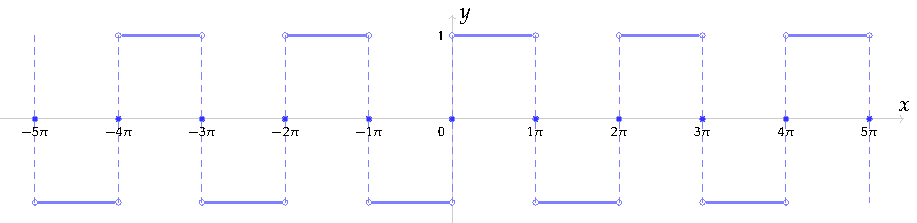
\includegraphics[width=14cm]{image/RecWave.pdf}
        \caption{方波的图像}
    \end{figure}
\end{frame}

\begin{frame}
    \frametitle{方波的傅里叶展开}
    \begin{itemize}
        \item 方波可以视为一个随时间变化的函数$f(x)$,有时为$1$,有时为$-1$。
        \item 方波亦可以视为一系列不同频率的正弦函数$\sin\omega x$按比例$F(\omega)$的叠加。
    \end{itemize}

    换言之,我们可以建立这样一种对应关系
    \begin{equation}
        f(x)\leftrightarrow F(\omega)=\frac{4}{\pi\omega},\quad\text{当$\omega$为奇数}
    \end{equation}
    其实,这就是傅里叶变换的核心思想。
\end{frame}

\begin{frame}
    \frametitle{傅里叶变换的核心思想}
    傅里叶变换的核心思想在于,同样一个函数(随时间变化的信号)
    \begin{itemize}
        \item 我们可以在时域$f\,(x)$上描述,即信号随时间如何变化。
        \item 我们可以在频率$F(\omega)$上描述,即信号中各个频率的简谐波的成分有多少。
    \end{itemize}
    傅里叶变换研究的,就是时域函数$f\,(x)$和频域函数$F(\omega)$之间如何转化。

    频域函数$F(\omega)$的实质,就是傅里叶级数中的“叠加系数”,但换了一种写法。
\end{frame}

\subsection{傅里叶变换}

\begin{frame}
    \frametitle{傅里叶级数到傅里叶变换}
    然而,要从傅里叶级数正式过渡到傅里叶变换,我们还要克服两个困难
    \begin{enumerate}
        \item 傅里叶级数的有正弦和余弦两套叠加系数,谁将作为频域函数?
        \item 傅里叶级数只能适用于周期函数,那非周期函数如何处理?
    \end{enumerate}
\end{frame}

\begin{frame}
    \frametitle{傅里叶级数的复数形式}
    根据傅里叶级数的展开式
    \begin{equation}
        f(x)
        =a_0+\Sum[n=1][\infty]{\qty[a_n\cos\frac{n\pi}{L}x+b_n\sin\frac{n\pi}{L}x]}
    \end{equation}
    运用欧拉公式
    \begin{equation}
        f(x)=a_0+\Sum[n=1][\infty]{\qty[
                    \frac{a_n}{2}\qty(
                    \e^{\i\frac{n\pi}{L}x}+
                    \e^{-\i\frac{n\pi}{L}x})+
                    \frac{b_n}{2\i}\qty(
                    \e^{\i\frac{n\pi}{L}x}-
                    \e^{-\i\frac{n\pi}{L}x})]}
    \end{equation}
\end{frame}

\begin{frame}
    \frametitle{傅里叶级数的复数形式}
    稍作整理
    \begin{equation}
        f(x)=a_0+\Sum[n=1][\infty]{\qty[
                    \frac{a_n-\i b_n}{2}
                    \e^{\i\frac{n\pi}{L}x}+
                    \frac{a_n+\i b_n}{2}
                    \e^{-\i\frac{n\pi}{L}x}]}
    \end{equation}
    我们期望的形式是
    \begin{equation}
        f(x)=\Sum[k=-\infty][\infty]{c_n\e^{\i\frac{k\pi}{L}x}}\qquad
        c_k=
        \begin{cases}
            \mal{\frac{a_n-\i b_n}{2}},&k>0,~n=+k\\[3mm]
            \mal{\frac{a_0}{2}},&k=0\\[3mm]
            \mal{\frac{a_n+\i b_n}{2}},&k<0,~n=-k
        \end{cases}
    \end{equation}
\end{frame}

\begin{frame}
    \frametitle{傅里叶级数的复数形式}
    分析系数
    \begin{align}
        a_0&=\frac{1}{2L}\Int[-L][L]{f(t)\dd{t}}\\[6pt]
        \frac{a_n-\i b_n}{2}
        &=\frac{1}{2L}
        \Int[-L][L]{f(t)\qty[\cos\frac{n\pi}{L}t-\i\sin\frac{n\pi}{L}t]\dd{t}}=
        \frac{1}{2L}
        \Int[-L][L]{f(t)\e^{-\i\frac{n\pi}{L}t}\dd{t}}\\[6pt]
        \frac{a_n+\i b_n}{2}
        &=\frac{1}{2L}
        \Int[-L][L]{f(t)\qty[\cos\frac{n\pi}{L}t+\i\sin\frac{n\pi}{L}t]\dd{t}}=
        \frac{1}{2L}
        \Int[-L][L]{f(t)\e^{\i\frac{n\pi}{L}t}\dd{t}}
    \end{align}
\end{frame}

\begin{frame}
    \frametitle{傅里叶级数的复数形式}
    因此,$c_k$的形式是统一的
    \begin{equation}
        c_k=\frac{1}{2L}
        \Int[-L][L]{f(t)\e^{-\i\frac{k\pi}{L}t}\dd{t}}
    \end{equation}
    至此,我们就成功的将傅里叶级数转换为了复数形式。
\end{frame}

\begin{frame}
    \begin{theorem}[傅里叶级数的复数形式]
        设$f(x)$是周期为$2L$的周期函数,即满足$f(x)=f(x+2L)$,且在$[-L,L]$上可积。

        若$f(x)$可以展开为以下形式的傅里叶级数
        \begin{equation}
            f(x)=\Sum[k=-\infty][\infty]{c_k\e^{\i\frac{k\pi}{L}x}}
        \end{equation}
        那系数$c_k$满足
        \begin{gather}
            c_k=\frac{1}{2L}
        \Int[-L][L]{f(t)\e^{-\i\frac{k\pi}{L}t}\dd{t}}
        \end{gather}
    \end{theorem}  
\end{frame}

\begin{frame}
    \frametitle{傅里叶变换的引入}
    \begin{center}
        非周期函数可以视为一个周期$L\to\infty$的周期函数。
    \end{center}
\end{frame}

\begin{frame}
    \frametitle{傅里叶变换的引入}
    \begin{center}
        傅里叶变换的实质,就是傅里叶级数的复数形式在周期$L\to\infty$的极限形态。
    \end{center}
\end{frame}

\begin{frame}
    \frametitle{傅里叶变换的引入}
    取傅里叶变换的复数形式$L\to\infty$的极限
    \begin{equation}
        f(x)=\Lim[L\to\infty]\Sum[k=-\infty][\infty]{c_k\e^{\i\frac{k\pi}{L}x}}
    \end{equation}
    引入代换变量
    \begin{equation}
        \omega=\frac{k\pi}{L}\qquad
        \delt{\omega}=\frac{\pi}{L}
    \end{equation}
    这里$\omega,\delt{\omega}$的意义是清楚的,$\omega$代表$k$时的频率,$\delt{\omega}$代表频率间隔。
\end{frame}

\begin{frame}
    \frametitle{傅里叶变换的引入}
    运用代换变量,$f(x)$的展开式可以改写为
    \begin{equation}
        f(x)=\Lim[L\to\infty]\Sum[k=-\infty][\infty]c_k\e^{\i\omega x}=\Lim[L\to\infty]\Sum[k=-\infty][\infty]\frac{Lc_k}{\pi}\e^{\i\omega x}\delt{\omega}
    \end{equation}
    而和式的极限,就是积分(当$L\to\infty$时有$\delt\omega\to 0$成立)
    \begin{equation}
        f(x)=\frac{1}{\pi}\Int[-\infty][\infty]\Lim[L\to\infty](Lc_k)\e^{\i\omega x}\dd{\omega}
    \end{equation}
\end{frame}

\begin{frame}
    \frametitle{傅里叶变换的引入}
    而$(Lc_k)$的在$L\to\infty$的极限很容易计算
    \begin{equation}
        \Lim[L\to\infty](Lc_k)=\Lim[L\to\infty]\qty(\frac{L}{2L}
        \Int[-L][L]{f(t)\e^{-\i\frac{k\pi}{L}t}\dd{t}})=\frac{1}{2}\Int[-\infty][\infty]f(t)\e^{-\i\omega t}\dd{t}
    \end{equation}
    如果我们记
    \begin{equation}
        F(\omega)=\frac{2}{\sqrt{2\pi}}\Lim[L\to\infty](Lc_k)=\frac{1}{\sqrt{2\pi}}\Int[-\infty][\infty]f(t)\e^{-\i\omega t}\dd{t}
    \end{equation}
    就有
    \begin{equation}
        f(x)=\frac{1}{\pi}\Int[-\infty][\infty]\Lim[L\to\infty](Lc_k)\e^{\i\omega x}\dd{\omega}=\frac{1}{\sqrt{2\pi}}\Int[-\infty][\infty]F(\omega)\e^{\i\omega x}\dd{\omega}
    \end{equation}
\end{frame}

\begin{frame}
    \begin{theorem}[傅里叶变换]
        设$f(x)$是定义在$(-\infty~~,\infty)$上的函数,并且在$(-\infty~~,\infty)$上绝对可积。

        那么定义$F(\omega)$为函数$f(x)$的傅里叶变换
        \begin{equation}
            F(\omega)=\frac{1}{\sqrt{2\pi}}\Int[-\infty][\infty]f(x)\e^{-\i\omega x}\dd{x}=\F{f(x)}
        \end{equation}
        其中$\e^{-\i\omega x}$称为傅里叶变换的核。而$f(x)$则称为函数$F(\omega)$的傅里叶逆变换
        \begin{equation}
            f(x)=\frac{1}{\sqrt{2\pi}}\Int[-\infty][\infty]F(\omega)\e^{\i\omega x}\dd{\omega}=\F*{F(\omega)}
        \end{equation}
        以上,将$F(\omega)$称为像函数,而将$f(x)$称为原函数。
    \end{theorem}  
\end{frame}

\begin{frame}
    \frametitle{傅里叶变换的一个重要性质}

    傅里叶变换有许多性质,这里我们要证明一个对今天的内容尤为重要的性质。

    \begin{theorem}[傅里叶变换的相似性质]
        设原函数$f(x)$,以及像函数$\F{f(x)}=F(\omega)$,对于任意实数$\lambda$,有
        \begin{equation}
            \F{f(\lambda x)}=\frac{1}{\abs{\lambda}}F\qty(\frac{\omega}{\lambda})
        \end{equation}
    \end{theorem}
\end{frame}

\begin{frame}
    \frametitle{傅里叶变换的一个重要性质}
    证明是容易的,根据傅里叶变换的定义
    \begin{equation}
        \F{f(\lambda x)}=\frac{1}{\sqrt{2\pi}}\Int[-\infty][\infty]{f(\lambda x)\e^{-\i\omega x}\dx}
    \end{equation}
    上式中作代换$\xi=\lambda x$,注意到$\dx=\dd{\xi}/\lambda$
    \begin{equation}
        \F{f(\lambda x)}=\frac{1}{\abs{\lambda}}\frac{1}{\sqrt{2\pi}}\Int[-\infty][\infty]f(\xi)\e^{-\i\frac{\omega}{\lambda}\xi}\dd{\xi}=\frac{1}{\abs{\lambda}}F\qty(\frac{\omega}{\lambda})
    \end{equation}
    上式出现$\abs{\lambda}$的原因是当$\lambda<0$时代换后积分限变为$(\infty,-\infty)$,而此时$\abs{\lambda}=-\lambda$。
\end{frame}

\begin{frame}
    \frametitle{傅里叶变换的一个重要性质}
    傅里叶变换的相似性质指出
    \begin{itemize}
        \item 时域上的压缩,在频域上表现为等比例的横向拉伸和纵向压缩。
        \item 时域和频域无法同时被压缩。
    \end{itemize}
\end{frame}